\chapter{LaTex笔记}
\section{每天日志格式}

%1.每天日志格式

1.每天日志格式
\begin{lstlisting}[]
\chapter{2020年3月3日} //1.以日期为章节
\section{问题1} //2.以问题为小节!
\end{lstlisting}

2.插入代码格式1
\begin{lstlisting}[]
\begin{lstlistings}[caption={xxx}] %插入图注 //默认是C语法
\end{lstlistings}
\end{lstlisting}

2.插入代码格式2
\begin{lstlisting}[]
\lstinputlisting{lbuf.c}[caption={xxx}] %插入图注!
\end{lstlisting}

2.插入代码格式3
\begin{lstlisting}[]
\lstinline !code!
\end{lstlisting}

3.插入图片格式
\begin{lstlisting}[]
\graphicspath{{note_everyday/001_20200302/picture/}} %声明图片加载路径
\begin{figure}[h] %h:表示把图片放在当前位置
    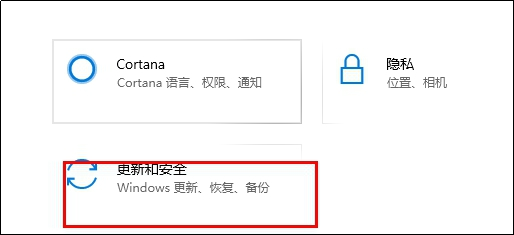
\includegraphics{001.jpg}
    \caption{第一步}
\end{figure}

\end{lstlisting}
